% Taken from https://github.com/mschroen/review_response_letter
% GNU General Public License v3.0

\documentclass[]{article}

\usepackage[includeheadfoot,top=20mm, bottom=20mm, footskip=2.5cm]{geometry}

% Typography
\usepackage[T1]{fontenc}
\usepackage{times}
%\usepackage{mathptmx} % math also in times font
\usepackage{amssymb,amsmath}
\usepackage{microtype}
\usepackage[utf8]{inputenc}

% Misc
\usepackage{graphicx}
\usepackage[hidelinks]{hyperref} %textopdfstring from pandoc
\usepackage{soul} % Highlight using \hl{}

% Table

\usepackage{adjustbox} % center large tables across textwidth by surrounding tabular with \begin{adjustbox}{center}
\renewcommand{\arraystretch}{1.5} % enlarge spacing between rows
\usepackage{caption}
\captionsetup[table]{skip=10pt} % enlarge spacing between caption and table

% Section styles

\usepackage{titlesec}
\titleformat{\section}{\normalfont\large}{\makebox[0pt][r]{\bf \thesection.\hspace{4mm}}}{0em}{\bfseries}
\titleformat{\subsection}{\normalfont}{\makebox[0pt][r]{\bf \thesubsection.\hspace{4mm}}}{0em}{\bfseries}
\titlespacing{\subsection}{0em}{1em}{-0.3em} % left before after

% Paragraph styles

\setlength{\parskip}{0.6\baselineskip}%
\setlength{\parindent}{0pt}%

% Quotation styles

\usepackage{framed}
\let\oldquote=\quote
\let\endoldquote=\endquote
\renewenvironment{quote}{\begin{fquote}\advance\leftmargini -2.4em\begin{oldquote}}{\end{oldquote}\end{fquote}}

% \usepackage{xcolor}
\newenvironment{fquote}
  {\def\FrameCommand{
	\fboxsep=0.6em % box to text padding
	\fcolorbox{black}{white}}%
	% the "2" can be changed to make the box smaller
    \MakeFramed {\advance\hsize-2\width \FrameRestore}
    \begin{minipage}{\linewidth}
  }
  {\end{minipage}\endMakeFramed}

% Table styles

\let\oldtabular=\tabular
\let\endoldtabular=\endtabular
\renewenvironment{tabular}[1]{\begin{adjustbox}{center}\begin{oldtabular}{#1}}{\end{oldtabular}\end{adjustbox}}


% Shortcuts

%% Let textbf be both, bold and italic
%\DeclareTextFontCommand{\textbf}{\bfseries\em}

%% Add RC and AR to the left of a paragraph
%\def\RC{\makebox[0pt][r]{\bf RC:\hspace{4mm}}}
%\def\AR{\makebox[0pt][r]{AR:\hspace{4mm}}}

%% Define that \RC and \AR should start and format the whole paragraph
\usepackage{suffix}
\long\def\RC#1\par{\makebox[0pt][r]{\bf RC:\hspace{4mm}}{\bf #1}\par\makebox[0pt][r]{AR:\hspace{10pt}}} %\RC
\WithSuffix\long\def\RC*#1\par{{\bf #1}\par} %\RC*
% \long\def\AR#1\par{\makebox[0pt][r]{AR:\hspace{10pt}}#1\par} %\AR
\WithSuffix\long\def\AR*#1\par{#1\par} %\AR*


%%%
%DIF PREAMBLE EXTENSION ADDED BY LATEXDIFF
%DIF UNDERLINE PREAMBLE %DIF PREAMBLE
\RequirePackage[normalem]{ulem} %DIF PREAMBLE
\RequirePackage{color} %DIF PREAMBLE
\definecolor{offred}{rgb}{0.867, 0.153, 0.153} %DIF PREAMBLE
\definecolor{offblue}{rgb}{0.0705882352941176, 0.168627450980392, 0.717647058823529} %DIF PREAMBLE
\providecommand{\DIFdel}[1]{{\protect\color{offred}\sout{#1}}} %DIF PREAMBLE
\providecommand{\DIFadd}[1]{{\protect\color{offblue}\uwave{#1}}} %DIF PREAMBLE
%DIF SAFE PREAMBLE %DIF PREAMBLE
\providecommand{\DIFaddbegin}{} %DIF PREAMBLE
\providecommand{\DIFaddend}{} %DIF PREAMBLE
\providecommand{\DIFdelbegin}{} %DIF PREAMBLE
\providecommand{\DIFdelend}{} %DIF PREAMBLE
%DIF FLOATSAFE PREAMBLE %DIF PREAMBLE
\providecommand{\DIFaddFL}[1]{\DIFadd{#1}} %DIF PREAMBLE
\providecommand{\DIFdelFL}[1]{\DIFdel{#1}} %DIF PREAMBLE
\providecommand{\DIFaddbeginFL}{} %DIF PREAMBLE
\providecommand{\DIFaddendFL}{} %DIF PREAMBLE
\providecommand{\DIFdelbeginFL}{} %DIF PREAMBLE
\providecommand{\DIFdelendFL}{} %DIF PREAMBLE
%DIF END PREAMBLE EXTENSION ADDED BY LATEXDIFF

% Fix pandoc related tight-list error
\providecommand{\tightlist}{%
  \setlength{\itemsep}{0pt}\setlength{\parskip}{0pt}}

% Add task difficulty and assignment commands from https://github.com/cdc08x/letter-2-reviewers-LaTeX-template
\usepackage[usenames,dvipsnames]{xcolor}
\usepackage{ifdraft}

\newcommand{\TaskEstimationBox}[2]{%
\ifoptiondraft{\parbox{1.0\linewidth}{\hfill \hfill {\colorbox{#2}{\color{White} \textbf{#1}}}}}%
{}%
}
%
\def\WorkInProgress {\TaskEstimationBox{Work in progress}{Cyan}}
\def\AlmostDone {\TaskEstimationBox{Almost there}{NavyBlue}}
\def\Done {\TaskEstimationBox{Done}{Blue}}
%
\def\NotEstimated {\TaskEstimationBox{Effort not estimated}{Gray}}
\def\Easy {\TaskEstimationBox{Feasible}{ForestGreen}}
\def\Medium {\TaskEstimationBox{Medium effort}{Orange}}
\def\TimeConsuming {\TaskEstimationBox{Time-consuming}{Bittersweet}}
\def\Hard {\TaskEstimationBox{Infeasible}{Black}}
%
\newcommand{\Assignment}[1]{
%
\ifoptiondraft{%
\vspace{.25\baselineskip} \parbox{1.0\linewidth}{\hfill \hfill \vspace{.25\baselineskip} \normalfont{Assignment:} \normalfont{\textbf{#1}}}%
}{}%
}


  \usepackage{tipa}
  \usepackage{booktabs}
  \usepackage{hyperref}
  \usepackage{longtable}


\newlength{\cslhangindent}
\setlength{\cslhangindent}{1.5em}
\newlength{\csllabelwidth}
\setlength{\csllabelwidth}{3em}
\newenvironment{CSLReferences}[2] % #1 hanging-ident, #2 entry spacing
 {% don't indent paragraphs
  \setlength{\parindent}{0pt}
  % turn on hanging indent if param 1 is 1
  \ifodd #1 \everypar{\setlength{\hangindent}{\cslhangindent}}\ignorespaces\fi
  % set entry spacing
  \ifnum #2 > 0
  \setlength{\parskip}{#2\baselineskip}
  \fi
 }%
 {}
\usepackage{calc}
\newcommand{\CSLBlock}[1]{#1\hfill\break}
\newcommand{\CSLLeftMargin}[1]{\parbox[t]{\csllabelwidth}{#1}}
\newcommand{\CSLRightInline}[1]{\parbox[t]{\linewidth - \csllabelwidth}{#1}\break}
\newcommand{\CSLIndent}[1]{\hspace{\cslhangindent}#1}

\begin{document}

{\Large\bf Author response to reviews of}\\[1em]
Manuscript APS-Feb-22-0015\\ \\
{\Large Using intonation to disambiguate meaning: The role of empathy and proficiency in L2 perceptual development}\\[1em]
{Joseph V. Casillas}\\
{submitted to \it Applied Psycholinguistics }\\
\hrule

\hfill {\bfseries RC:} \textbf{\textit{Reviewer Comment}}\(\quad\) AR: Author Response \(\quad\square\) Manuscript text

\vspace{2em}

Dear XXX,

Thank you for taking the time to consider our manuscript \emph{Using intonation to disambiguate meaning: The role of empathy and proficiency in L2 perceptual development
} (APS-Feb-22-0015) for publication in \emph{Applied Psycholinguistics}.
Our understanding is that we needed to consider the reviewers' comments and revise accordingly before the manuscript could be reevaluated for publication.
We have considered thoroughly the detailed feedback provided by all three reviewers and resubmit what we believe to be a much improved version of the manuscript.
In this letter we address the reviewers' concerns point-by-point.
Where feasible, we quote all revised text in this document, otherwise, we refer the reader to the relevant lines in the revised manuscript.
We thank you and the 3 anonymous reviewers for all comments and suggestions and again enthusiastically submit the revised manuscript for consideration in \emph{Applied Psycholinguistics}.

Sincerely,\\
Joseph Casillas\\
(corresponding author)

\clearpage

\hypertarget{reviewer-1}{%
\section{Reviewer \#1}\label{reviewer-1}}

\hypertarget{introduction-and-objectives}{%
\subsection{INTRODUCTION AND OBJECTIVES}\label{introduction-and-objectives}}

\RC{The terms perception, processing and comprehension are used in the manuscript not very systematically. 
In some cases the authors use “perception and processing” together, and in some others they seem to summarize them both in the term “comprehension”. 
A more systematic use of these terms is needed.}

We thank the reviewer for their comment.
In the revised manuscript we have tried to be consistent with how the terms are implemented in the phonetics/phonology, SLA, and psycholinguistic literatures.
We reserve the term `comprehension' to refer to one's general understanding of linguistic input (see Esteve-Gibert et al., 2020 for examples).
In the majority of cases we have simplified the revised manuscript by opting for `perception'/`speech perception', which we use to refer to the ability to perceive linguistic structure in the speech signal.
We make a distinction between general `perception' and `sentence processing' when we refer to comprehension at the sentence-level and specifically to insight derived from online tasks (reaction times, eye-tracking gaze data, etc.) as opposed to response accuracy.
We believe these distinctions have been made more explicit throughout the revised manuscript.
We have opted not to explicitly operationalize these terms in the prose, as we believe they are generally understood by the readership of Applied Psycholinguistics, though we are happy to be more explicit at the discretion of the editor.

\Done
\Easy

\RC{The authors used distinct terms to refer to the same sentence type: absolute interrogative, polar question, yes/no question, total interrogative... 
It also alternates between the term ‘statement’ and the term ‘declarative’. 
It recommends using one term in a systematic way and to describe and exemplify what these terms mean for readers that are not experts on intonation (or syntax or pragmatics). 
The authors now provide some general description of the intonational patterns in the introduction (e.g. ‘nuclear hat pattern’, ‘final rise’, but I doubt whether a reader that is not an expert on intonation will understand these descriptions).}

This observation was also pointed out by reviewer 2 and duly noted.
We have systematized our use of these terms in the revised manuscript.
When we refer to questions (generally), we now say interrogative utterances, and, more specifically, `yes/no questions' and `wh- questions' instead of `absolute interrogatives' and `partial interrogatives', respectively.
When we refer to declarative utterances (generally) we now say `declarative statements', and, more specifically, `broad focus statements' and `narrow focus statements'.
These changes are also reflected in all plots and tables, as well as the supplementary materials.

\Done

\RC{The introduction mentions several times that “intonation may result in comprehension and communication difficulties” and that “interpreting L2 intonation is challenging”, and it feels a bit repetitive. 
These statements should also be better motivated and better justified (intonation more than other linguistic aspects? 
which kind of difficulties? what does ‘challenging’ mean? 
why is it challenging? all intonation patterns work equally?).}

We thank the reviewer for their suggestion.
In the revised manuscript we have reduced the amount of times this point is emphasized to avoid repetition and in the referred text we have avoided describing the learning process as ``difficult'' or ``challenging'' because at this juncture of the introduction we are not interested in comparing the relative difficulty of different linguistic elements, nor explaining how different intonation patterns might cause more or less problems.
Instead, our aim is illustrate that semantic meaning mapping is language-specific and that L2 learners typically have non-target-like outcomes due to cross-linguistic influence.
We believe we have made this point more clear in the revised manuscript.
We include the relevant text below for convenience.

\begin{quote}
This is, in part, because in everyday discourse speakers can use intonation to indicate syntactic structure, to signal whether an utterance is a question or a statement, to focus constituents, as well as to convey affective meaning.
Notably, the manner in which intonation is mapped to meaning is often language-specific.
As a consequence, L2 intonation is often produced in a non-target-like fashion due to cross-linguistic influence.

Intonation has a semantic function and through adequate cognitive decoding of the signal a listener can interpret the intended meaning of a given utterance.
For example, an intonational contour can indicate to a listener whether the utterance of an interlocutor is a question or a statement.
As touched upon above, a speaker can use prosody to signal numerous additional pragmatic functions as well.
This rich variation in pragmatic uses makes the interpretation and decoding of intonational contours during speech comprehension a non-trivial task for the language learner.
Moreover, the use of first language (L1) prosodic features when speaking the target language can result in misunderstandings because the same prosodic features can convey different linguistic and paralinguistic meaning in the target language (Chen, 2005; Cruz-Ferreira, 1987; Mennen, 2007; Pickering, 2001).
As noted by Levis (2016), prosody is also ``{[}\ldots{]} critical for L2 pronunciation because it plays a major role in cementing social bonds as a key marker of social identity'' (p.~154).
\end{quote}

\Done
\Easy

\RC{The factor “speaker dialectal variety” seems to appear and disappear from the manuscript. The introduction includes a paragraph on dialectal variance in Spanish intonation, and it is included as a third research question, but the authors should elaborate further on why dialectal variance may affect the processing of L2 intonation or even if it may affect learning. In the discussion and conclusion this factor is not mentioned when the authors summarize the aims of the study at the beginning of these sections. In sum, one feels that this research question is not well integrated into the study (or at least the manuscript).}

In the revised manuscript the topic of speaker variety is reported in the results section on pages 25-26 and we dedicate 4 paragraphs of the discussion section to possible explanations for our findings (approx. pp.~32-34).
We hope that the reviewer finds this to be sufficient.
Furthermore, at the request of this reviewer (see below) and reviewer 2, we provide more detail regarding self-reported familiarity with Spanish.
This information is also included in the discussion section and the supplementary materials.

\Done
\Easy

\RC The study explores 4 specific sentence types that differ at the intonation level. The authors should motivate the selection of these sentence types, describe them at the intonational level for all varieties used, and elaborate on why certain sentence types are more difficult to process for L2 learners and, more specifically, for English learners of Spanish. Otherwise it is not possible to understand the nature of the differences that had to be perceived by the participants of the study and that, more generally, have to be learned in an L2.

At the recommendation of all three reviewers we have included more information about the stimuli used in our study (please see the introduction section and the supplementary materials, as it is too much information to include here).
The 4 sentence types, while not exhaustive, were selected for two reasons.
First, they are the most commonly analyzed utterances in the intonational phonology literature.
Thus, these tunes represent the intonational contours about which we know the most.
Second, these are the sentence types (and the exact sentences) used in Brandl, González, and Bustin (2020), which our study replicates conceptually.

\Done
\Easy

\RC{Also, why empathy should play a role in how these specific sentence types are perceived and processed? Why do the authors think that the listeners’ ability to feel/think what the other feel/think may impact in distinguishing questions from statements? In other words: what are the intonational cues in a declarative or in a yes/no question that may lead to distinct processing accuracy and speech by listeners with distinct empathy skills? Please motivate these aspects further.}

These are excellent questions.
We appreciate the reviewer's critical eye in pointing out these missing elements in our motivation of empathy.
We have included more information in the introduction to address these points.
The basic idea proceeds as follows.
From the perspective of the listener, empathy is likely critical because it allows one to understand the intentions of others, predict their behavior, and understand their emotions (Baron-Cohen \& Wheelwright, 2004).
Researchers that work on this construct have described two types of empathy that oftentimes might be difficult to distinguish.
\emph{Affective empathy} represents one's ability to be emotionally aligned with the interlocutor and \emph{cognitive empathy} refers to recognizing and understanding the feelings and thoughts of an interlocutor.
Thus, we believe empathy, to some degree, is a necessary element when an individual seeks to understand and interact with its interlocutors.

When we apply this to everyday communication, we find that speakers' expressions and feelings cannot be limited to only lexical or semantic cues.
Speakers employ other strategies, such as using intonational cues, with the intention of producing a meaningful expressions that can include pragmatic connotations, and mental states, among other meaningful expressions.
For instance, speakers can signal pragmatic information via pitch accents.
A high tone at the end of a phrase can signal a yes/no question the same way as a final high tone preceded by a rising pitch accent can indicate unexpected information (in Spanish).
The extant literature suggests that individual pragmatic skills modulate intonation processing (Bishop, 2016; Bishop, Chong, \& Jun, 2015; Bishop \& Kuo, 2016; Diehl, Bennetto, Watson, Gunlogson, \& McDonough, 2008).
The critical studies in the case that concerns us are Esteve-Gibert, Portes, Schafer, Hemforth, and D'Imperio (2016), Esteve-Gibert et al. (2020), and Orrico and D'Imperio (2020), which suggest that individuals with higher empathy (operationalized as a pragmatic skill) may be better at processing intonation-meaning associations.

Importantly, \emph{why} and \emph{how} particular acoustic cues lead to distinct processing outcomes on the part of the listener is still unclear.
A priori, one would have reason to believe that the effects of empathy on processing intonation-meaning associations would be present across the board, i.e., for any utterance type.
In our data, we find that higher empathy is moderately associated with higher accuracy (holding proficiency constant) for all utterance types, with the exception of yes/no questions.
Importantly, this also happens to be the most difficult utterance condition in our data---and that of Brandl et al. (2020)---as well as the condition for which the listeners show the least sensitivity (See d' analysis in the supplementary materials).
At this juncture, our focus is on expanding this line of research in two ways: (1) to individuals with different linguistic experience (specifically, second language learners), and (2) to different communicative/pragmatic situations (utterance types).
We are not concerned (yet) with understanding \emph{why} different pitch contours affect intonation perception, particularly with regard to the role of empathy, because there is inherent variability in how speakers realize their communicative intentions, at the variety-level and at the individual-level, within utterance types.
This variability is present in our stimuli.
We believe a fruitful avenue for future research is to explore \emph{why} and \emph{how} particular acoustic realizations of pitch within utterance types lead to distinct processing outcomes, though this is not the specific goal of this paper.

In the revised manuscript we have expanded on these issues in both the introduction and the discussion sections.
We do not copy the revised text here due to excessive length, but we direct the reviewer's attention to approximately p.~10, and p.~37.

\Done
\Easy

\RC{Please elaborate and motivate further why you think that empathy may lead to higher/faster intonational development in an L2 (expectation for RQ2). Likewise, please motivate further your expectations for RQ3, as they are now somehow disconnected from the literature reviewed in the introduction. The authors mention that statements might be more difficult to differentiate from questions in the Cuban variety, but without information on why this must be the case (a distinct intonational pattern for certain questions, maybe?) it is impossible to evaluate whether this expectation makes sense.}

We thank the reviewer for this comment.
Given that there is no research that we know of regarding empathy and L2 perceptual development, our motivation is based solely on findings from studies on monolinguals.
The logic is the following.
Recent studies related to monolingual sentence processing find that empathy influences speech perception (Esteve-Gibert et al., 2016, 2020; Orrico \& D'Imperio, 2020).
This line of work operationalizes the construct empathy as a pragmatic skill and has focused on it as a source of individual differences.
To elaborate on just one example, Esteve-Gibert et al. (2020) shows that listeners with different levels of empathy interpret intonation and meaning in contexts in which a temporary lexical ambiguity could only be resolved through intonation.
The higher empathy group was more sensitive to intonation cues in the process of forming sound-meaning associations.
In other words, they used intonation to resolve temporary lexical ambiguities.
As mentioned, there is limited research in SLA involving empathy, and there are no studies, as far as we know, dealing with empathy and L2 speech perception.
That being said, if empathy plays a role in monolingual sentence processing, a valid question is to ask if this is also the case in second language sentence processing.
We have tried to make this clear in the revised manuscript and include below a relevant section illustrating the logic explained above.

\begin{quote}
The particular body of work linking empathy with SLA has focused on speech production, or, more specifically, on what early scholars considered `authentic pronunciation' and, more recently, `pronunciation aptitude' (See Rota \& Reiterer, 2009), though no strong associations have been found.
To the best of our knowledge, no studies have explored the construct empathy as it pertains to L2 perceptual development.
Thus, at this time we do not know if empathy plays a role in L2 sentence processing in a similar manner to monolingual sentence processing.
The present project extends this research to the SLA context to determine if individual differences in this pragmatic skill affect the development of intonation in L2 perception and sentence comprehension.
\end{quote}

With regard to research question 3, our hypothesis that learners will have more difficulty with the Cuban variety is grounded in our pilot data with monolingual Spanish speakers.
We found that participants were much less accurate in the 2afc task when responding to the stimuli provided by the Cuban speaker (and to a lesser extent the Puerto Rican speaker).
A priori we would have had no justification for this hypothesis had we not collected the pilot data.
In hindsight, it would have made sense to pre-register a hypothesis stating that participants would be more accurate responding to speakers of varieties with which they were more familiar.
However, we would not have been able to answer this question---at least not to the extent one would hope---as the listeners in the data we collected mainly stated being most familiar with U.S. Spanish (See pp.~32-33 for brief discussion).
We now offer an additional plausible explanation based on familiarity with Spanish.\\
Specifically, we analyzed the data from the participants who claimed to be most familiar with a Spanish variety that was included in our speaker varieties: Peninsular and Mexican Spanish (note: we make the assumption that `Peninsular' is most closely associated with the Madrileño speaker).
We coded the participants' responses to familiar versus unfamiliar varieties and fit a Bayesian logistic regression model to the data (complete details provided in the manuscript).
In short, we find that, marginalizing over proficiency and empathy, participants were indeed more accurate when responding to a familiar variety.
This is true for all utterance types to some degree, but more clearly the case for questions (likely because responses to declarative utterances were near ceiling).
Figure \ref{fig:plot-learner-variety-familiarity} and Table \ref{tab:table-learner-variety-familiarity-conditional-effects} below illustrate the familiarity effect and are now included in the discussion section and supplementary materials.

\clearpage



\begin{figure}
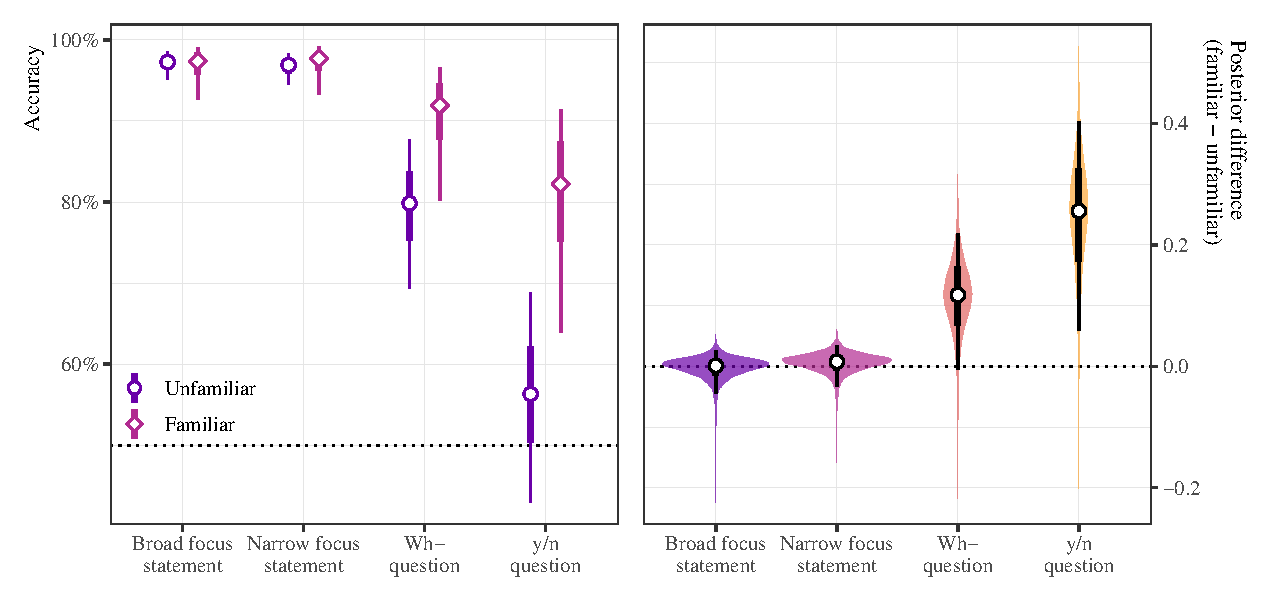
\includegraphics[width=1\linewidth]{../../../../figs/manuscript/learner_variety_familiarity} \caption{Response accuracy as a function of utterance type for unfamiliar and familiar Spanish varieties. Values represent posterior medians along with the 95\% HDI for unfamiliar and familiar conditions (left panel), as well as the posterior difference (familiar - unfamiliar; right panel). The posterior predictive distribution is based on data from 91 participants who claimed to be familiar with Mexican (n = 47) and Peninsular (n = 44) Spanish.}\label{fig:plot-learner-variety-familiarity}
\end{figure}

\begin{longtable}[]{@{}lrrr@{}}
\caption{\label{tab:table-learner-variety-familiarity-conditional-effects}Conditional effects of response accuracy as a
function of sentence type and familiarity with the Spanish variety.
Values represent posterior medians along with the 95\% HDI for unfamiliar
and familiar conditions, along with the posterior difference
(familiar - unfamiliar). The posterior predictive distribution is based on
data from 91 participants
who claimed to be familiar with Mexican (n = 47)
and Peninsular (n = 44) Spanish.}\tabularnewline
\toprule()
Sentence type & Unfamiliar & Familiar & Difference \\
\midrule()
\endfirsthead
\toprule()
Sentence type & Unfamiliar & Familiar & Difference \\
\midrule()
\endhead
Broad focus statement & 0.97 {[}0.95, 0.99{]} & 0.97 {[}0.94, 0.99{]} & 0.00 {[}-0.04, 0.03{]} \\
Narrow focus statement & 0.97 {[}0.95, 0.99{]} & 0.98 {[}0.95, 1.00{]} & 0.01 {[}-0.03, 0.04{]} \\
Wh- question & 0.80 {[}0.70, 0.88{]} & 0.92 {[}0.83, 0.97{]} & 0.12 {[}0.00, 0.22{]} \\
y/n question & 0.56 {[}0.43, 0.69{]} & 0.82 {[}0.67, 0.93{]} & 0.26 {[}0.07, 0.41{]} \\
\bottomrule()
\end{longtable}

Finally, we have expanded on the motivation for our hypothesis in the revised manuscript and also included our exploratory analyses of the pilot data in the discussion section and the supplementary materials.
This was the only motivation for this hypothesis and precisely what was preregistered prior to collecting any data.
Copied below is the relevant change to the introduction.

\begin{quote}
Finally, with regard to RQ3, we hypothesize that, overall, L2 learners will have the most difficulty (lower accuracy, slower response time) with the Cuban variety.
This hypothesis is grounded in exploratory analyses of pilot data collected from 120 monolingual Spanish speakers in which responses to the Cuban variety were the least accurate (See Supplementary Materials for more information).
\end{quote}

\Done
\Easy

\hypertarget{stimuli}{%
\subsection{STIMULI}\label{stimuli}}

\RC{Details on the stimuli used for the experimental task are much needed. Please describe the sentences used at the acoustic and phonological level, for all varieties, and provide a list of these sentences. Importantly, were they controlled at the syntactic and lexical levels to ensure that potential differences in processing speed were not due to syntactic or lexical factors? On a related note, and crucially to interpret your results, how can we be sure that listeners responded based on the intonational cues they perceived and not on potential syntactic and lexical cues in the sentences?}

We have included acoustic and phonological descriptions of the stimuli along with a complete list of items in the supplementary materials of the revised manuscript.
All items within an utterance type followed the same syntactic structure, with the exception of the wh- questions, which require a wh- word.
In theory, the presence alone of the wh- word could sway the listener to believing they are hearing a question, however, these words are also present in statements.
The intonational contour is necessary for one to differentiate between the two.
Importantly, the participants were generally not accurate for either question type (approx. 63\% for yes/no questions and approx. 72\% wh- questions, marginalizing over proficiency and empathy).
We provide an example in Table \ref{tab:item-ex-table}.

\footnotesize

\begin{longtable}[]{@{}llll@{}}
\caption{\label{tab:item-ex-table}Example stimuli from the 2AFC task.}\tabularnewline
\toprule()
Utterance type & Prompt & Item & Translation \\
\midrule()
\endfirsthead
\toprule()
Utterance type & Prompt & Item & Translation \\
\midrule()
\endhead
Broad focus statement & n/a & \emph{Marta abre el regalo} & Marta opens the gift. \\
Narrow focus statement & ¿Qué abre Marta? & \emph{Marta abre el regalo} & (What does Marta open?) Marta opens the gift. \\
Wh- question & n/a & \emph{¿Por qué abre el regalo?} & Why does she open the gift? \\
y/n question & n/a & \emph{¿Marta abre el regalo?} & Does Marta open the gift? \\
\bottomrule()
\end{longtable}

\normalsize

\Done
\Easy

\RC{Please provide the results of the 100 monolingual Spanish speakers rating the quality of items.}

The data from 120 monolingual Spanish speakers were used to pilot the items/task.
In other words, these listeners did not rate the quality of the items.
We have included our exploratory analyses of the pilot data in the supplementary materials.
As mentioned previously, accuracy was high (lowest for the Cuban and Puerto Rican varieties when responding to questions).
Unsurprisingly (though of interest), when looking at the monolingual listeners' accuracy when responding to stimuli from their own variety, e.g., Andalusian listeners responding to stimuli from the Andalusian speaker, accuracy was at ceiling for all the variety matches for which we have data (Andalusian, Chilean, Cuban, Madrileño, Mexican, and Puerto Rican).

\Done
\Easy

\RC{Please provide details on which variety the listeners were familiar with, and put these data in relation to the participants' responses in the results in a more systematic way.}

This issue was addressed above (See Figure \ref{fig:plot-learner-variety-familiarity} and Table \ref{tab:table-learner-variety-familiarity-conditional-effects}) and has been included in the revised manuscript and the supplementary materials.

\Done
\Easy

\hypertarget{results-discussion}{%
\subsection{RESULTS \& DISCUSSION}\label{results-discussion}}

\RC{Results show that proficiency and empathy interact in wh-questions but not in yes/no questions or declaratives, and that empathy had an effect in all sentence types except for yes/no question. There is no discussion on how these findings relate to previous literature on sentence comprehension, or even on what may originate these differences across sentence types. Instead, the discussion and conclusion now seem to mask these differences across sentence types.}

In the revised manuscript we have focused our discussion on what we believe to be the most relevant studies with regard to sentence comprehension and empathy.
We have also expanded our discussion concerning why we don't find an effect for empathy with regard to yes/no questions.
Of particular interest to the reviewer are pages 31-33.
For convenience, we include relevant excerpts below.

\begin{quote}
In line with previous studies (e.g., Brandl et al., 2020), we found that yes/no questions were most difficult for L2 learners of Spanish, followed by wh- questions and broad focus and narrow focus statements.
An exploratory analysis using d' found that learner sensitivity to the utterance types followed the same pattern.
While it is not clear exactly why yes/no question are the most difficult, one possibility is that wh- questions pose less of a challenge because they contain a wh- word (e.g., \emph{cuándo}, \emph{cómo}, etc.).
In other words, it might be the presence of a lexical cue in our task (and that of Brandl et al., 2020) that facilitates the interpretation of a wh- question in addition to intonation.
At this juncture this possibility cannot be discarded, though it is worth noting that the presence of these words alone does not imply a question.
That is to say, in specific contexts these same words appear in statements as well, e.g., \emph{Que bebe María}, \emph{Que beba María}, etc.
A specific intonation contour is obligatory to force a question interpretation.
Moreover, apart from the propositional content, a wh- question also implies a presupposition, and, thus, is more pragmatically complex.
On the other hand, the yes/no questions in our experimental task have the same syntactic structure as the declarative statements.
Perhaps for this reason yes/no questions require more effort and attention to intonation in order to distinguish them from statements in our task.
\end{quote}

As well as\ldots{}

\begin{quote}
Additionally, our study addressed the question \emph{Do pragmatic skills---specifically, empathy---modulate the rate of development in L2 prosody?}
This question was motivated by a line of research showing that empathy influences language processing in monolingual populations (Esteve-Gibert et al., 2016, 2020; Orrico \& D'Imperio, 2020).
Though the construct \emph{empathy} has been considered in the SLA literature, the current body of research is limited to studies on pronunciation accuracy (i.e., Guiora, Brannon, \& Dull, 1972; Rota \& Reiterer, 2009, among others).
Thus, we extend research on empathy to L2 phonological acquisition as it relates to speech perception.
Using a cross-sectional design, we show (1) that empathy, as measured by the empathy quotient (Baron-Cohen \& Wheelwright, 2004), did indeed modulate response accuracy and the decision-making process, and (2) \emph{how} empathy affected sentence processing was related to L2 proficiency.
Specifically, we found response accuracy increased as a function of proficiency, independent of empathy for yes/no questions, but not wh- questions.
In the case of the latter, we found empathy to have a compounding effect on the correlation between accuracy and proficiency, such that higher empathy individuals showed more accuracy at lower proficiency levels when compared with their lower empathy counterparts.
This is taken as evidence suggesting that pragmatic skill can modulate the rate of development in L2 prosody.
That is to say, higher empathy individuals may develop L2 prosody at an earlier stage than lower empathy individuals.
That being said, we do not find the same effect with yes/no questions.
This finding is quite puzzling, particularly because previous research on sentence processing has found an effect for empathy in yes/no questions, e.g., in Salerno Italian (Orrico \& D'Imperio, 2020).
At this time, we are uncertain as to why our results differ in this regard, though the nature of the outcome variable measured in the task used in Orrico and D'Imperio (2020) (certainty scores bounded at 0 and 100) may have provided a more fine-grained window into the effect of empathy.
\end{quote}

\Done
\Easy

\RC Could you check whether individuals with higher empathy were not the ones with higher proficiency? How did these two factors correlate?

The relationship between empathy and proficiency is estimated in a number of ways.
First, the effect of the interaction between the two predictors on response accuracy is estimated for each utterance type and are reported in the manuscript.
Second, our model also estimated this correlation in the grouping effects and provided no compelling evidence that the two predictors are correlated (\(\beta\) = 0.056, HDI = {[}-0.403, 0.494{]}, ROPE = 0.326, MPE = 0.589).
Specifically, we can see that the most plausible estimate is quite small, that the distribution of plausible values is quite wide, and that there is only approximately a 58\% chance the correlation is positive (it is almost equally likely to be negative).
Thus, we feel confident that the participants with higher proficiency are not necessarily the same ones with higher empathy.

\Done
\Easy

\RC{In the discussion the authors highlight the fact that proficiency was treated as a continuous variable, and the reader would benefit from knowing whether this is actually an innovation of the present study or if, instead, other studies have done it before (now it seems that it is an innovation).}

The use of proficiency as a continuous variable is not an innovation of our study.
The reason continuous variables are discretized in other research likely results from the choice of analysis, e.g., analysis of variance (ANOVA), which requires a continuous outcome variable be predicted by factors (categorical variables).
While we do believe that the common practice of discretization of continuous variables is less than ideal, it is not our intention to speak to this topic in the manuscript.
The description regarding how the variable is coded is included (a) for the sake of completeness and reproducibility, and (b) to highlight our departure from Brandl et al. (2020), which our study replicates conceptually.

\Done
\Easy

\RC{The authors try to explain the variety-specific responses by providing three hypotheses. However, I think that none of these hypotheses are sufficiently motivated or explained. First, they state that “familiarity with the target variety may account for variety-specific response accuracy”, although this cannot be derived from the results you obtained since most of your listeners were most familiar with US Spanish (which was not in the stimuli). Second, they state that they may derive from the fact that distinct varieties produce each sentence type using distinct intonational patterns, although it is impossible to evaluate if this hypothesis is plausible because details on the intonational features of the stimuli are missing and because results are never matched to the nature of the contour that was perceived. Finally, the authors propose an explanation linked to the distinct speech rate used in distinct varieties. The authors should provide a detailed description of the speech rate of the stimuli, by variety, in order for the reader to be able to evaluate if this explanation is indeed plausible. All in all, I recommend the authors to adjust the discussion of the effect of listener/speaker variety to the results that were actually obtained, and to provide enough details of the stimuli to ensure the reader can assess the validity of these explanations.}

We thank the reviewer for this comment.
Respectfully, we believe the reviewer may has missinterpreted our intentions in this section of the discussion.
We are not providing hypotheses with the intention of testing them, but rather we are proving plausible explanations for what we have found in our study.
Our pre-registered hypotheses are explained in the introduction and revisited in light of the results in the discussion.
Having said that, we would like to address the three points made by the reviewer.
The reviewer states:

\textbf{"First, they state that “familiarity with the target variety may account for variety-specific response accuracy”, although this cannot be derived from the results you obtained since most of your listeners were most familiar with US Spanish (which was not in the stimuli)."}

We agree with the reviewer that we cannot determine this with the data we have collected.
We did not anticipate that our learners would identify U.S. Spanish as the variety they were most familiar with as frequently as they did.
Nonetheless, we did include a familiarity analysis based on a subset of the data (See explanation above, as well as Figure \ref{fig:plot-learner-variety-familiarity} and Table \ref{tab:table-learner-variety-familiarity-conditional-effects}).
This information has been included in the discussion of the revised manuscript and additional details are available in the supplementary materials.

\textbf{"Second, they state that they may derive from the fact that distinct varieties produce each sentence type using distinct intonational patterns, although it is impossible to evaluate if this hypothesis is plausible because details on the intonational features of the stimuli are missing and because results are never matched to the nature of the contour that was perceived."}

Again, we would like to stress that this is not a hypothesis we intend to test in our project.
We are primarily focused on how pragmatic meaning is inferred with regard to proficiency and empathy.
We put forth the aforementioned explanation for this very reason.
Future research should control the pitch contours of the utterance types in order to say \emph{why}/\emph{how} certain contours may (or may not) be more difficult than others.
Nonetheless, we have included extensive acoustic detail regarding our stimuli, which are freely available for future researchers to use.

\textbf{"Finally, the authors propose an explanation linked to the distinct speech rate used in distinct varieties. The authors should provide a detailed description of the speech rate of the stimuli, by variety, in order for the reader to be able to evaluate if this explanation is indeed plausible."}

We agree with the reviewer that more information regarding the speech rate of each variety should have been included.
The revised manuscript includes more detail, particularly Table \ref{tab:table-stimuli-sr} and Figure \ref{fig:plot-sm-random-speech-rate}, which we also include here for convenience.

\begin{longtable}[]{@{}lrrr@{}}
\caption{\label{tab:table-stimuli-sr}Average articulation rate (number of syllables divided by total
phonation time), syllable duration (in milliseconds), and speech rate (number
of syllables divided by total time) for each variety of the acoustic stimuli
presented to listeners.}\tabularnewline
\toprule()
Variety & Articulation rate & Syllable duration & Speech rate \\
\midrule()
\endfirsthead
\toprule()
Variety & Articulation rate & Syllable duration & Speech rate \\
\midrule()
\endhead
Andalusian & 3.75 & 288 & 3.72 \\
Argentine & 3.59 & 300 & 3.59 \\
Madrileño & 3.72 & 282 & 3.72 \\
Chilean & 3.95 & 264 & 3.95 \\
Cuban & 3.99 & 272 & 3.99 \\
Mexican & 4.51 & 230 & 4.51 \\
Peruvian & 3.70 & 286 & 3.70 \\
Puerto Rican & 4.02 & 277 & 4.02 \\
\bottomrule()
\end{longtable}



\begin{figure}
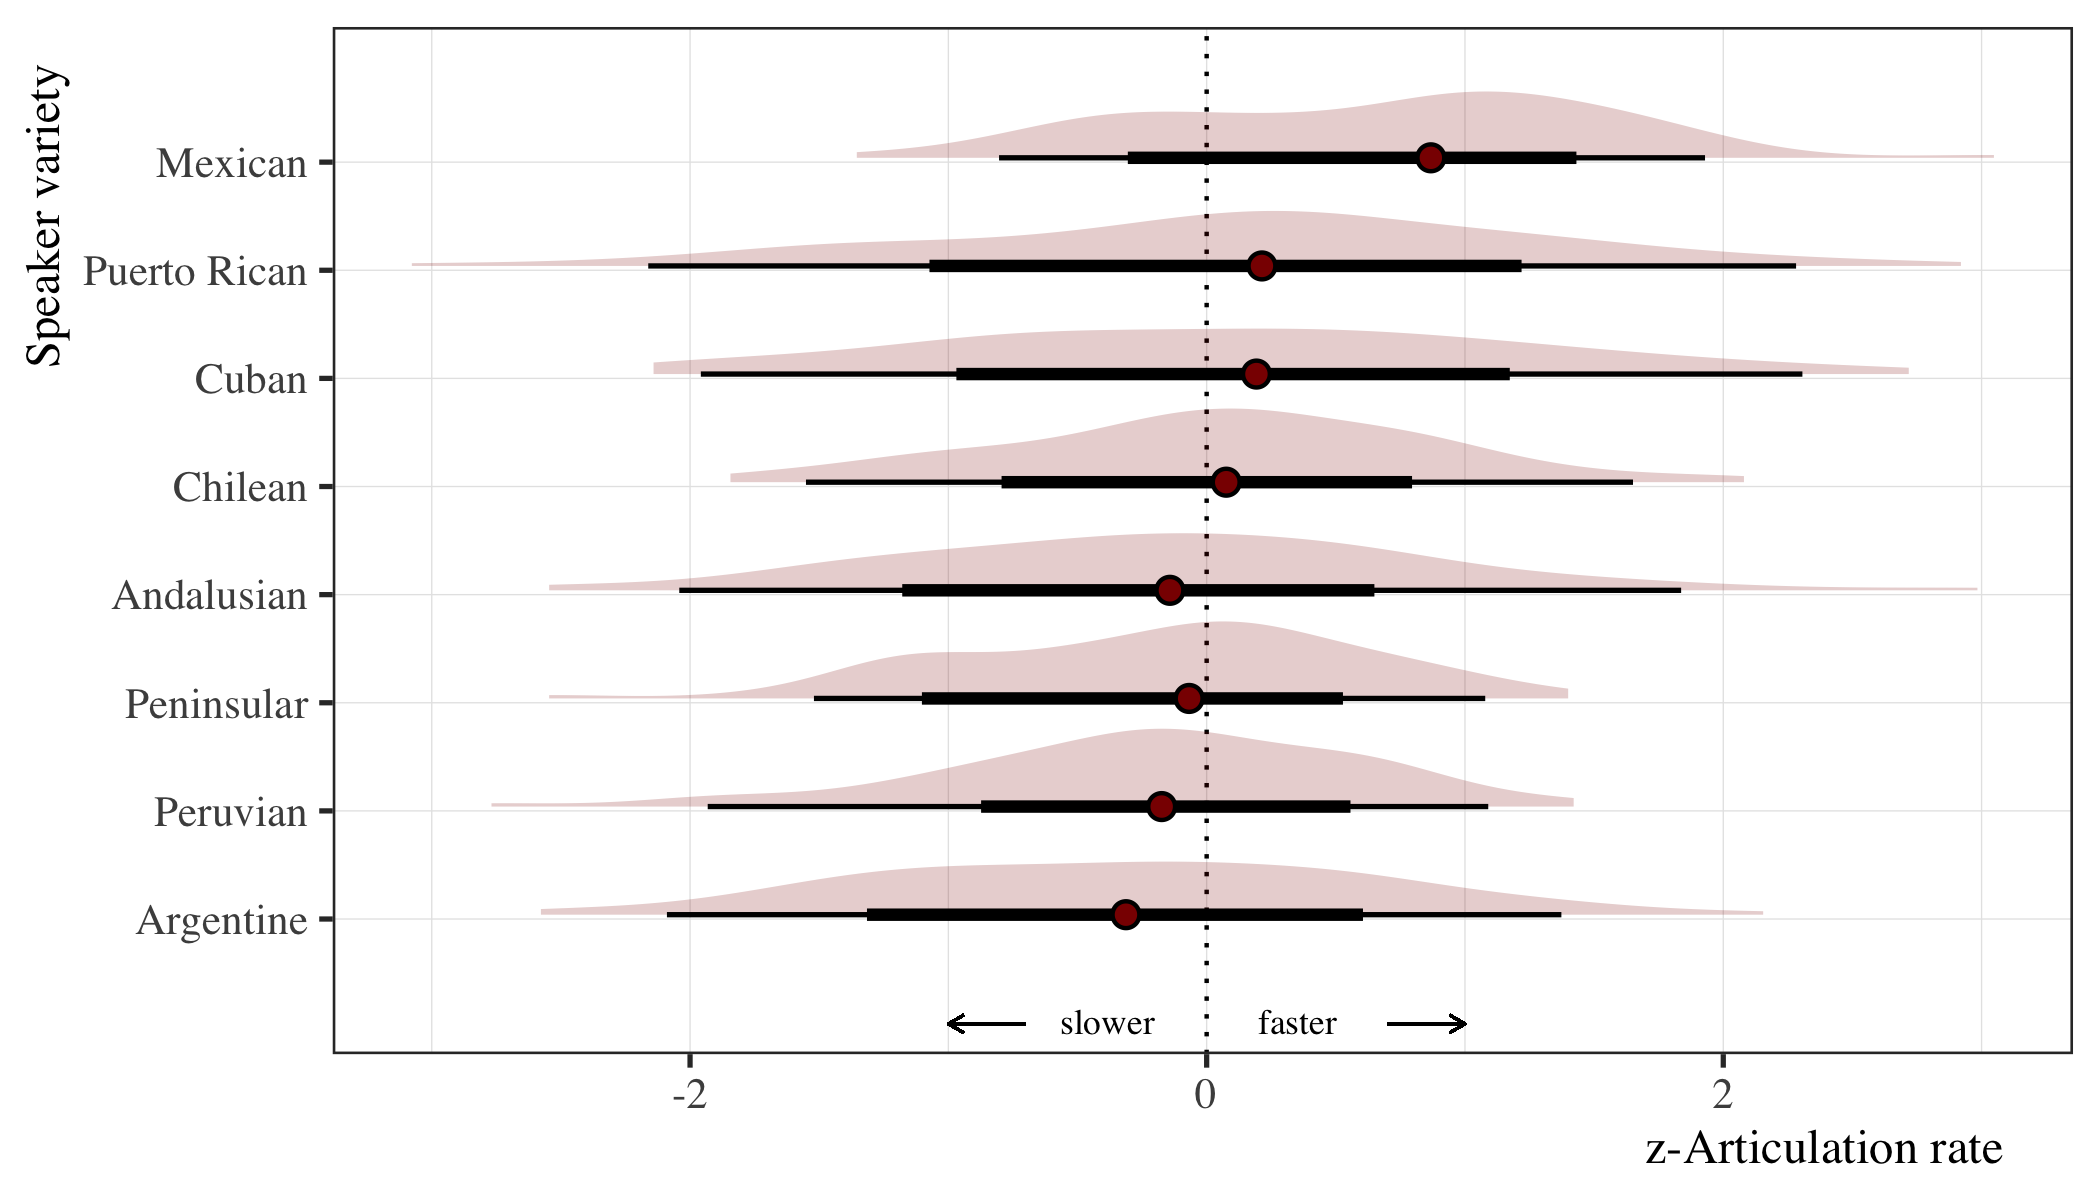
\includegraphics[width=1\linewidth]{../../../../figs/manuscript/sm_speech_rate} \caption{Standardized articulation rate as a function of speaker variety. Points represent posterior medians along with 66\% and 95\% HDI.}\label{fig:plot-sm-random-speech-rate}
\end{figure}

\Done
\Easy

\clearpage

\hypertarget{reviewer-2}{%
\section{Reviewer \#2}\label{reviewer-2}}

\hypertarget{comments-to-the-author}{%
\subsection{Comments to the Author}\label{comments-to-the-author}}

\RC This is a very interesting study looking at the roles of proficiency and empathy in the development of L2 prosodic perception. The authors use sophisticated statistical methods to show that both proficiency and empathy seem to be at play in the development of L2 prosodic perception, as well as the specific type of prosody. The paper also considers the role of dialect, which is very often not dealt with in studies of L2 prosody. In paying attention to these aspects of prosodic acquisition, the paper is cutting edge. I think that the paper would benefit from a clear theoretical model with specific predictions based on that model, and perhaps the authors can investigated whether Mennen's LiLT model would help them do that or not. Below I present some general recommendations, followed by some specific comments.

We thank the reviewer for these kind words and their insightful comments, which we have responded to below.
We are confident that the revised manuscript is much stronger after taking them into consideration.

\Done
\Easy

\hypertarget{recommendations}{%
\subsection{Recommendations:}\label{recommendations}}

\RC{I would like to see more discussion about proficiency which as I understand was really about vocabulary. What do the authors think the relationship between vocabulary size and prosodic comprehension is? It would be interesting to see more discussion of this in the paper, since the authors made a decision to measure “proficiency” in this way. Is it that learners might be acquiring more “things” overall? More words but also more tunes? This could be explored further.}

We thank the reviewer for this comment.
The LexTALE measures vocabulary size as a proxy for general proficiency.
This assumption is based on evidence reported in Lemhöfer and Broersma (2012), who found that L2 English speakers performance on the LexTALE was correlated with their English vocabulary size and general proficiency, and was overall a better predictor of language proficiency than self-ratings.
In our case, we expected (and found) an association between higher general proficiency and prosodic development (an increase in LexTALE score was be associated in general with a higher probability of a correct response), and this general finding is consistent with Brandl et al. (2020) using an experimental paradigm similar to the one we use.
There are also many studies in the SLA/Bilingualism literature that use the LexTALE in a similar way (Garrido Pozú, 2022 for recent examples; see Lozano-Arg\&uuml;elles et al., 2021).
While we completely agree that it would be interesting to explore the relationship between growing vocabulary size and specific tunes, we believe this is beyond the scope of this paper.
We are primarily concerned with using vocabulary size as a proxy for general proficiency, which allows us to control this variable and explore how it interacts with empathy.

\Done
\Easy

\RC{As mentioned in the detailed comments, I don’t think it makes sense to conflate empathy and “pragmatic skills”. I know the authors claim that they are “operationalizing” empathy as pragmatic skills, but I don’t see a need to do this. While being highly empathetic might and probably does play a role in one’s pragmatic skills, I don’t think it makes sense to say they are the same thing. I think the authors can simply talk about empathy and leave it there, which is what they are doing in the analysis anyway.}

This issue is referenced several times.
We respond here and subsequent comments refer back to this response.
As we understand it, the reviewer's comments touch on two important issues: (1) whether or not empathy is a pragmatic skill itself and (2) whether our study has anything to do with pragmatic skills in the firstplace.
First, empathy has previously been treated as a pragmatic skill in recent studies.
Esteve-Gibert et al. (2020) explain that empathy is part of the set of pragmatic abilities known as theory of mind, and they add that empathy is one of the pragmatic skills that enable listeners to understand the communicative intentions encoded in the interlocutor's words.
Their research found that listeners with better pragmatic skills (i.e., higher empathy) are more sensitive to intonation cues when forming sound-meaning associations and using intonation to disambiguate meaning.
We operationalized empathy as a pragmatic skill following Esteve-Gibert et al. (2020), whose stance follows research in psychology on the construct (See Baron-Cohen, 2011; Carruthers, 2009; Frith \& Frith, 2003).
We agree that empathy ``{[}\ldots{]} is part of the set of pragmatic abilities that enable listeners to understand the communicative intentions and feelings behind the interlocutor's words (Baron-Cohen \& Wheelwright, 2004)'' (p.~577).
We accept that the reviewer may not agree with this particular operationalization.
That being said, we don't believe that implementing it affects the main points of our manuscript.
Given that our study builds upon the findings of Esteve-Gibert et al. (2020) and builds upon their findings, we feel it is appropriate to operationalize empathy as a pragmatic skill to be consistent with the previous research.
Second, regardless of whether we agree that empathy is a pragmatic skill itself or an ability that helps pragmatic skills/pragmatic reasoning, as the reviewer suggests, our study does indeed relate to how pragmatic skills are used to interpret meaning through intonation.
Therefore we be believe a discussion about pragmatic skills is warrented in the context of our study.
As we discuss in the manuscript, previous research has reported that speakers make use of intonational cues of speech to express pragmatic meaning, mental states, among others, and to structure information in speech (See also Esteve-Gibert et al., 2020; Ladd, 2008; Prieto, 2015).
In our experimental task, participants were required to decide whether the utterances they listened to were questions or statements solely on the basis of the intonation they perceived, which directly taps into their pragmatic abilities (including empathy).
According to Esteve Gibert et al.~(2020), empathy is a pragmatic skill that allows listeners to interpret the intentions behind the interlocutor's message, which is exactly the focus of our study.

\Done
\Easy

\RC{This is also mentioned in the more detailed comments, but I would like to see some sort of description of the tunes (at least the nuclear configurations) for each variety and sentence type. At the very least a very phonetic description would do (e.g. a rise to a high tone in the nuclear stressed vowel, followed by a fall to a low boundary tone). But I think this would make for a better discussion of the findings. This might also help the authors to make sense of the finding about wh-questions and the role of proficiency and empathy for those. Why wh-questions?}

\WorkInProgress
\Easy

\RC{While the paper points out the need for L2 models to account for levels further than the segment, the paper doesn’t make any suggestions about how to do so and does not mention the most recent proposal of a model for L2 intonation. Please check the following for the model more generally: 

Mennen, I. (2015). Beyond segments: Towards a L2 intonation learning theory. In E. Delais-Roussaire, M. Avanzi, \& S. Herment (Eds.), Prosody and language in contact (pp. 171–188). Heidelberg, Germany: Springer

And specifically for the case of Spanish:

Sánchez Alvarado, Covadonga. 2020. The production and perception of subject focus prosody in L2 Spanish. University of Massachusetts Amherst dissertation. 

Alvarado, Covadonga Sánchez and Armstrong, Meghan. "Prosodic Marking of Object Focus in L2 Spanish" Studies in Hispanic and Lusophone Linguistics, vol. 15, no. 1, 2022, pp. 211-250. <https://www.degruyter.com/document/doi/10.1515/shll-2022-2060/html>
}

We were unaware of Mennen's model and these additional references.
We thank the reviewer for bringing them to our attention.
We have included a brief summary of the model in the introduction of the revised manuscript (and revisit the model in the discussion).
We include the relevant portion referenced in the reviewer's comment below:

\begin{quote}
Research on L2 intonation has been concerned primarily with speech production.
Learner difficulties tend to be ascribed to L1 transfer, and models of L2 phonology, by and large, focus on the speech segment, as in the Speech Learning Model revised (Flege \& Bohn, 2021), or contrasts between segments, i.e., PAM-L2, L2LP (Best \& Tyler, 2007; Van Leussen \& Escudero, 2015, respectively).
Theoretical work centered on prosody in the acquisition of L2 phonology is relatively much less common, though some researchers have considered how the aforementioned models might account for suprasegmental phenomena (See Trofimovich \& Baker, 2006).
One clear example of this is the L2 Intonation Learning Theory (LILt, Mennen, 2015).
LILt incorporates the basic assumptions of the SLM and PAM-L2, that L2 categories similar to L1 categories may be assimilated, but L2 categories that are perceptually different may be incorporated as new categories.
Under this model, cross-language differences may occur along one or more intonation dimensions (systemic, realizational, semantic, and frequency) (See also Ladd, 2008) and the age of onset of acquisition may influence the degree of success in acquiring elements in different dimensions of language variation.

A dearth of knowledge remains regarding how perception of intonation develops in L2 learning, and even less is known about how individual pragmatic differences account for learner outcomes.
Similar to the SLM, LILt focuses mostly on intonation production rather than perception, and adopts the assumption that difficulties in intonation production are perceptually motivated.
The purpose of the present project is to address this gap in the literature by examining the perception of intonation during adult L2 phonological acquisition.
For the present study, investigating L2 perception of intonation in statements and questions in L2 learners of Spanish provides an opportunity to examine how L2 perception develops and may differ from L1 perception, especially along the `semantic dimension' of the LILt model, which focuses on how intonation is used to convey meaning.
Importantly, whereas LILt considers the influence of external factors such as age of acquisition on the success of learners, the present study investigates the role of empathy as a pragmatic skill on L2 acquisition of intonation, which contributes to our understanding of intonation development along a different dimension.
\end{quote}

MUST ADD TO DISCUSSION TOO. STILL IN PROGRESS

\WorkInProgress
\Easy

\RC{p. 3, line 23-29 - Please also include literature on information structure (focus, givenness, etc.) as well as speaker belief states
}

\WorkInProgress
\Easy

\RC{p. 4, 47-50 - I think it could be useful to include some concrete examples of the various meanings here, to demonstrate the plethora of meanings that can arise
}

\WorkInProgress
\Easy

\RC{p. 5, 23-29 - Also reference the discussion regarding the instruction of prosody in Durwing \& Monroe 2015
}

This reference has been included in the revised manuscript.

\Done
\Easy

\RC{p. 6,paragraph beginning on line 47 - there should be some mention of Mennen’s LiLT (L2 intonational learning theory) model of L2 intonation and the recent work using this model
}

\WorkInProgress
\Easy

\RC{p. 6 line 39 - both Caribbean Spanish and Argentine (porteño?) Spanish use final f0 falls for yes-no questions (absolute interrogatives), I’m not sure this description actually captures the differences. Also, there are differences in the actual falls in different Caribbean Spanishes. Varieties of DR Spanish use what is best described as H+L* L% while Puerto Rican Spanish uses ¡H* L%. I think Hualde & Prieto also shows that question falls are actually rather common in Spanish, even if their pragmatic meanings are more restricted. 
}

\WorkInProgress
\Easy

\RC{The author(s)might consider using the term polar or yes/no questions throughout, since these terms are more accessible outside the Hispanic Linguistics lit, which tends to use “absolute interrogatives”.}

Following this suggestion and that of reviewer 1, we have systematized how we refer to all utterance types throughout the revised manuscript.
We now refer to absolute interrogatives as `yes/no questions'.

\Done
\Easy

\RC{p. 9 line 4 - has empathy been “operationalized as pragmatic skill” in the past? Is it really possible to say that they are the same thing, vs. one leading to the other? 
}

We have responded with more detail to this issue above.
To the point brought up here, indeed, there is a line a research that operationalizes empathy as a pragmatic skill (Baron-Cohen, 2011; See Baron-Cohen \& Wheelwright, 2004; Carruthers, 2009; Esteve-Gibert et al., 2020; Frith \& Frith, 2003, among others).

\Done
\Easy

\RC{p. 10 - line 45 - perceptional—> perceptual??}

We thank the reviewer for pointing out this oversight.
This mistake has been fixed in the revised manuscript.

\Done
\Easy

\RC{research question 2 - Again, it’s hard for me to buy empathy AS a pragmatic skill itself. I would say it’s an ability that could be helpful for pragmatic skills/pragmatic reasoning. But not the same thing. If the authors disagree I’d like to see this justified more. Given what the study does, I’m not sure you have to say anything about pragmatic skills at all, you can just call it empathy.}

We refer the reviewer to our previous comment on this issue, which we addressed here.

\Done
\Easy

\RC{p. 11, line 8, again, why not just call them yes-no questions?}

This issue was addressed previously.
We include our response again here for the sake of completeness.

Following this suggestion and that of reviewer 1, we have systematized how we refer to all utterance types throughout the revised manuscript.
We now refer to absolute interrogatives as `yes/no questions'.

\Done
\Easy

\RC p.~15, line 25 - I'm wondering what perceptual learning would mean here. We know that the encoding of narrow focus and question intonation differs across the varieties that are listed here. How would we know if these participants had experience with these varieties? It would be helpful to know what the tunes for each type of sentence were for each variety used in the stimuli as well.

\WorkInProgress
\Easy

\RC p.~26, lines 53-6 (on next page)- I'm not sure this makes sense'' In practical terms, this implies that high proficiency, high empathy learners required more information to reach a decision and responded at a slower rate, particularly with regard to low empathy learners (top row), regardless of proficiency level.''
Do they mean ``compared'' to low empathy learners (as opposed to ``particularly with regard to low empathy learners'')?

We did indeed mean to say ``compared'' to lo empathy learners.
This has been changed in the revised manuscript.

\Done
\Easy

\RC p.~29, line 28 - ``This is taken as evidence suggesting that pragmatic skill can modulate the rate of development in L2 prosody.'' again, I don't see a reason to call this pragmatic skill. It's just empathy. better to say - ``That is to say, higher empathy individuals may develop L2 prosody at an earlier stage than lower empathy individuals.''

As mentioned previously, this issue is addressed HERE.
In this particular instance, we have opted to replace ``pragmatic skill'' with ``empathy'' in the revised manuscript.
\Done
\Easy

\RC p.~31 - line 5 - The idea that there is one ``US Spanish'' is very controversial. US Spanishes still have the characteristics of the varieties of origin, so even though respondents are familiar with Spanish spoken in the U.S. they would be exposed to Mexican Spanish, Dominican Spanish, Puerto Rican Spanish, etc. as spoken in the US. Looking at which region of the country respondents were from could be helpful in understanding this.

\WorkInProgress
\Easy

\RC p.~31 - line 20 - The authors discuss the possibilities of why the different varieties might have been perceived differently. I think it would be helpful for the authors to share what the tunes in their stimuli actually were, which would help them to better surmise here. Puerto Rican Spanish (not mentioned in the discussion) and Cuban Spanish were the varieties people had the most difficulties with, but according to most descriptions PRS and CS use the same tune for ys questions (also again, NB that Dominican ynqs are not the same as PRS and CS ynqs, this description conflates all Caribbean Spanish questions, which are also not necessarily hat patterns). I would recommend an appendix with a description of the tunes in the stimuli for each variety, and for this to be brought into the discussion for research question \#3.

\WorkInProgress
\Easy

\RC p.~32, line 7 - again, the LiLT model needs to be mentioned, since this reads as if no theory of L2 intonation has been proposed.

\WorkInProgress
\Easy

\clearpage

\hypertarget{reviewer-3}{%
\section{Reviewer \#3}\label{reviewer-3}}

\hypertarget{comments-to-the-author-1}{%
\subsection{Comments to the Author}\label{comments-to-the-author-1}}

\RC{The study analyses the influence of empathy in the perception and processing of intonation in questions and statements in L2 Spanish and shows that higher empathic individuals, in comparison with lower empathic individuals, appear to be more sensitive to intonation cues. In my opinion, the quality of the paper is very good and the conclusions make it a highly citable one and not only for the case of Spanish L2 but in general. 

Below you can find a by-section review and some comments.

The goals and hypothesis of the paper are clear and well-defined.
}

\WorkInProgress
\Easy

\RC{As for the state of the art, page 29, line 6 states: "the current body of research is limited to studies on pronunciation accuracy." And I think that is not accurate, there are studies that include empathy as an important factor for intonation perception (in L1 and mostly from psychology that is true) \href{https://journals.plos.org/plosone/article?id=10.1371/journal.pone.0008759}{[Link]}

And, then, specifically for Spanish L2, a recent poster presented in New Sounds 2022 uses the Autism Spectrum Quotient (I don't know if they publish abstracts as short papers) \href{https://www.researchgate.net/publication/361371026_The_Role_of_Native_Language_Experience_and_Individual_Features_in_the_Cross-linguistic_Perception_of_Spanish_Intonation}{[Link]}

Maybe you can add this info in the introduction stating that it is a very recent and promising field of research and that it helps us to understand individual variation and that way you won't need to change much in your text.
}

\WorkInProgress
\Easy

\RC The methodology of the paper is outstanding, a great sample size (225 listeners), good materials (with several Spanish varieties included) and a state-of-the-art statistical analysis for fussy reviewers and an innovative one (at least for our discipline), that I don't fully understand, so maybe it is a good idea to organize a workshop on that in a future congress.

\WorkInProgress
\Easy

\RC I have only have questions regarding those ``64 critical items'' that (I think) can be easily solved including examples or a description of the patterns the speakers used or better (and you will see why in the comments) how you elicited the data and saying something like ``variation is wonderful, students must be exposed to a wide range of intonational patterns and we are not interested in their pragmatic meaning for this study''.

\WorkInProgress
\Easy

\RC First, silly question, why do the listeners need intonation in wh- questions? They have the marker ``qué, quién, cómo''\ldots{} That is all they need, so I don't understand why this type of question is included in the study.

\WorkInProgress
\Easy

\RC I know that the stimuli are in the supplementary materials, but I miss something in the text either an example (or two of them) or making explicit of the type of stress that you have included and why. The reason is that a lot of foreign speakers (that is the case for example for Dutch, Japanese and Chinese if I remember it correctly) find more difficult to distinguish between statements and questions when the last word of the sentence is stressed in the last syllable (aguda). And that has two main reasons, 1) compression and truncation of the tonal movements and 2) (and of special importance given the varieties included among your stimuli) most of Mexican, Peninsular Spanish, Chilean, Peruvian statements can be slightly rising. In pragmatic descriptions such as Prieto \& Roseano (2010) that final contour is characterised as ``statement of the obvious'' but, in fact, that is the pattern that we find most of the times that we elicit statements that have the slightest hint of common ground information, for example, in narratives. Moreover, in some varieties of Mexico and Chile, slightly rising (L* !H\%) is the standard neutral pattern. This has a direct implication in the perception of questions by native speakers that counterintuitively, need a higher F0 rise in order to say that something is a question than foreigners that speak usually speak languages where there are not rising statements (I would give you references but they are mine, so maybe when the paper is published, we can talk in a congress). Maybe you don't find that because English-speaking speakers are used to uptalk?

\WorkInProgress
\Easy

\RC Before I start criticizing your stimuli in the follow paragraphs, I want you to know that I very much appreciate that you made them public and that if every researcher did this we will find problems in every dataset. So, this does not diminish your work at all. Now, some of the things that I am going to say are not solvable in a reviewed version and I am aware of that, and I do not expect you to solve them, the paper is publishable as long as you include the sentence that I said before saying that the sentences have several contours and several pragmatic meanings.

\WorkInProgress
\Easy

\RC Firstly, eliciting real broad-focus sentences is not easy and not only because the tendency to the statement of the obvious, for example, your andalusian\_match\_declarative-broad-focus\_David-leia-el-libro has a slightly (but audible and present in the pitch contour) narrow-focus intonation (rising stressed syllable) and the only narrow-focus that I could find among all your stimuli. So, maybe we are calling narrow-focus to different things, let me know if we are.

\WorkInProgress
\Easy

\RC{As for the wh- questions, Spanish has loads of patterns, for example in Argentina wh- questions can be rising or falling depending on politeness, in Peninsular Spanish are usually falling but they can be rising, and usually is the same for any dialect. And, then we have all the biased intonation patterns, for example, your Andalusian speaker is using the "surprised one" L+H\*L\%, which happens to coincide with the pattern for focus, in all the wh- questions except in "andalusian\_match\_interrogative-partial-wh\_Por-que-ama-la-navidad", where she uses the L\*H\%, the prototypical one for yes-no questions in standard Castilian Spanish.

For the rest, most of your speakers have chosen rising patterns for their wh-questions but that is not the most frequent pattern.
}

\WorkInProgress
\Easy

\RC As for focus, all your speakers should be doing a rising stressed syllable and falling ending (L+H* L\%), that is pretty much panhispanic and crosslinguistically really frequent. But they are not, the case of the Peruvian speaker is salient because is using a monotonous tone, just the opposite of what she should be doing.

\WorkInProgress
\Easy

\RC In the case of the Argentinian speaker if you look at the sentences side by side you will see that in the supposedly narrow sentence the peak is a bit earlier but it is still in the post-stressed syllable. We will expect here the Argentinian narrow-focus pattern, which is the most recognizable thing of their accent and the only case in which Spanish has a tritonal accent L+H*+L (peak in the middle of the stressed syllable surrounded by low tones).

\WorkInProgress
\Easy

\RC{And then your Andalusian speaker has been innovative and has chosen for most of the cases the statement of the obvious pattern (realised as L\*H\%) therefore using the y-n question pattern. The context that Prieto and Roseano (2010) have for that is:
A: ¿De quién es el hijo?
B: ¡De quién va a ser! de Guillermo
So for your data would be something like: A: María bebe el vino. (while she is thinking: obvio, ¿por qué me lo preguntas?)
}

\WorkInProgress
\Easy

\RC In the rest of them I think that she is trying to put the focus on the verb, but the result is really strange. To do that, you would need something like ``Mariano HAbla \textbar{} del tiempo (and does not another thing)'' and you will have a small pause with compressed post-focal material etc. What she does is just weird.

\WorkInProgress
\Easy

\RC And lastly, yes-no questions, in general rising (here the Andalusian speaker is using the Madrid standard Spanish), but falling in Cuba, Puerto Rico, all the Caribbean, North of Spain, Canary Islands\ldots{} The good thing is that the falling patterns that you have are not easily mistaken with a statement (for example questions of Medellín (Colombia) are) and the bad thing again is that you have more than one pattern.

\WorkInProgress
\Easy

\RC Ok, so the message after this is that the choice of a pattern by the speakers has made that some of the stimuli are more difficult that others and that maybe you could solve that by adding a new variable ``pattern used'', which for most of the cases will be the interaction between variety and utterance type but for those speakers that use different patterns it won't. In fact, if you redo the analysis in order to see the effect of the contour, I would use this variable instead of utterance type because most of the supposedly narrow-focus sentences are broad-focus and will share the L*L\% contour. And again, I am not saying that you do that for the current paper, you can prepare a new experiment to focus on intonational patterns.

\WorkInProgress
\Easy

\RC{Results. Nothing to say, beautifully solved, I loved the inclusion of speech rate as a variable that could affect the results. 

Congratulations on your work and I hope to see the reviewed version soon.
}

\WorkInProgress
\Easy

\newpage

From Hualde and Prieto (2015)

Andalusian
- Sosa (1999)
- Henriksen and García-Amaya (2012)

Argentine
- Sosa (1999)
- Colantoni and Gurlekian (2004)
- Colantoni (2011)
- Labastía (2006)
- Labastía (2011)

Chilean
- Ortiz-Lira and Cid-Uribe (2000)
- Ortiz-Lira (2003)

Cuban
- Sosa (1999)
- Alvord (2006)

Madrileño
- Quilis (1981)
- Quilis (1987)
- Quilis (1993)
- Sosa (1999)
- Estebas-Vilaplana and Prieto (2010)

Mexican
- Quilis (1981)
- Quilis (1987)
- Quilis (1993)
- Sosa (1999)
- Sosa (2003)
- Butragueño (2003)
- Butragueño (2004)

Peruvian
- Sosa (1999)
- O'Rourke (2005)

Puerto Rican
- Quilis (1981)
- Quilis (1987)
- Quilis (1993)
- Sosa (1999)
- Sosa (2003)
- Armstrong (2010)
- Armstrong (2012)

\newpage

\hypertarget{references}{%
\section{References}\label{references}}

\hypertarget{refs}{}
\begin{CSLReferences}{1}{0}
\leavevmode\vadjust pre{\hypertarget{ref-alvord2006spanish}{}}%
Alvord, S. M. (2006). \emph{Spanish intonation in contact: The case of {M}iami {C}uban bilinguals} (PhD thesis). University of Minnesota.

\leavevmode\vadjust pre{\hypertarget{ref-armstrong2010puerto}{}}%
Armstrong, M. E. (2010). Puerto {R}ican {S}panish intonation. In P. Prieto \& P. Roseano (Eds.), \emph{Transcription of intonation of the {S}panish language} (pp. 155--189). Münich: Lincom Europa.

\leavevmode\vadjust pre{\hypertarget{ref-armstrong2012development}{}}%
Armstrong, M. E. (2012). \emph{The development of yes-no question intonation in {P}uerto {R}ican {S}panish} (PhD thesis). The Ohio State University.

\leavevmode\vadjust pre{\hypertarget{ref-baron2011zero}{}}%
Baron-Cohen, S. (2011). \emph{Zero degree of empathy. On empathy and the origins of cruelty}. London, England: Penguin.

\leavevmode\vadjust pre{\hypertarget{ref-baron2004empathy}{}}%
Baron-Cohen, S., \& Wheelwright, S. (2004). The empathy quotient: An investigation of adults with {A}sperger syndrome or high functioning autism, and normal sex differences. \emph{Journal of Autism and Developmental Disorders}, \emph{34}(2), 163--175. \url{https://doi.org/10.1023/B:JADD.0000022607.19833.00}

\leavevmode\vadjust pre{\hypertarget{ref-Best2007}{}}%
Best, C. T., \& Tyler, M. D. (2007). Nonnative and second-language speech perception: {C}ommonalities and complementarities. In O.-S. Bohn \& M. J. Munro (Eds.), \emph{Language experience in second language speech learning: {I}n honor of {James Emil Flege}} (pp. 13--34). Amsterdam, The Netherlands: John Benjamins.

\leavevmode\vadjust pre{\hypertarget{ref-bishop2016individual}{}}%
Bishop, J. B. (2016). Individual differences in top-down and bottom-up prominence perception. \emph{Proceedings of Speech Prosody}, \emph{2016}, 668--672.

\leavevmode\vadjust pre{\hypertarget{ref-bishop2015individual}{}}%
Bishop, J. B., Chong, A. J., \& Jun, S.-A. (2015). Individual differences in prosodic strategies to sentence parsing. \emph{Proceedings of the 18th International Congress of Phonetic Sciences}, 1--5. London: International Phonetic Association.

\leavevmode\vadjust pre{\hypertarget{ref-bishop2016autistic}{}}%
Bishop, J. B., \& Kuo, G. (2016). Do {``autistic-like''} personality traits predict prosody perception. \emph{Talk Presented at LabPhon15 Satellite Workshop on Personality in Speech Perception and Production, Ithaca, NY}.

\leavevmode\vadjust pre{\hypertarget{ref-bustin_2020}{}}%
Brandl, A., González, C., \& Bustin, A. (2020). The development of intonation in {L}2 {S}panish: {A} perceptual study. In A. Morales-Front, M. J. Ferreira, R. P. Leow, \& C. Sanz (Eds.), \emph{Hispanic linguistics: Current issues and new directions} (pp. 12--31). John Benjamins Publishing Company. \url{https://doi.org/10.1075/ihll.26}

\leavevmode\vadjust pre{\hypertarget{ref-butragueno2003hacia}{}}%
Butragueño, P. M. (2003). Hacia una descripción prosódica de los marcadores discursivos. {D}atos del español de {M}éxico. \emph{La Tonía: Dimensiones Fonéticas y Fonológicas}, 375--402.

\leavevmode\vadjust pre{\hypertarget{ref-butragueno2004configuraciones}{}}%
Butragueño, P. M. (2004). Configuraciones circunflejas en la entonación del español mexicano. \emph{{R}evista de {F}ilología {E}spañola}, \emph{84}(2), 347--373.

\leavevmode\vadjust pre{\hypertarget{ref-carruthers2009we}{}}%
Carruthers, P. (2009). How we know our own minds: The relationship between mindreading and metacognition. \emph{Behavioral and Brain Sciences}, \emph{32}(2), 121--138. \url{https://doi.org/10.1017/S0140525X09000545}

\leavevmode\vadjust pre{\hypertarget{ref-chen2005universal}{}}%
Chen, A. (2005). \emph{On the universal and language-specific perception of paralinguistic intonational meaning}. Utrecht: LOT.

\leavevmode\vadjust pre{\hypertarget{ref-colantoni2011broad}{}}%
Colantoni, L. (2011). \emph{Broad-focus declaratives in {A}rgentine {S}panish contact and non-contact varieties}. John Benjamins.

\leavevmode\vadjust pre{\hypertarget{ref-colantoni2004convergence}{}}%
Colantoni, L., \& Gurlekian, J. (2004). Convergence and intonation: Historical evidence from {Buenos Aires Spanish}. \emph{Bilingualism: Language and Cognition}, \emph{7}(2), 107--119. \url{https://doi.org/10.1017/S1366728904001488}

\leavevmode\vadjust pre{\hypertarget{ref-cruz1987}{}}%
Cruz-Ferreira, M. (1987). Non-native interpretive strategies for intonational meaning: An experimental study. In A. James \& J. Leather (Eds.), \emph{Sound patterns in second language acquisition} (pp. 103--120). Berlin: Mouton de Gruyter.

\leavevmode\vadjust pre{\hypertarget{ref-diehl2008resolving}{}}%
Diehl, J. J., Bennetto, L., Watson, D., Gunlogson, C., \& McDonough, J. (2008). Resolving ambiguity: {A} psycholinguistic approach to understanding prosody processing in high-functioning autism. \emph{Brain and Language}, \emph{106}(2), 144--152. \url{https://doi.org/10.1016/j.bandl.2008.04.002}

\leavevmode\vadjust pre{\hypertarget{ref-estebas_prieto2010}{}}%
Estebas-Vilaplana, E., \& Prieto, P. (2010). Castilian {S}panish intonation. In P. Prieto \& P. Roseano (Eds.), \emph{Transcription of intonation of the {S}panish language} (pp. 17--48). Münich: Lincom Europa.

\leavevmode\vadjust pre{\hypertarget{ref-esteve2016role}{}}%
Esteve-Gibert, N., Portes, C., Schafer, A., Hemforth, B., \& D'Imperio, M. (2016). \emph{The role of individual empathic skills on the online processing of intonational meaning}. Bilbao, Spain: Basque Center on Cognition, Brain; Language. \url{https://doi.org/10.13140/RG.2.2.19401.13926}

\leavevmode\vadjust pre{\hypertarget{ref-esteve2020empathy}{}}%
Esteve-Gibert, N., Schafer, A. J., Hemforth, B., Portes, C., Pozniak, C., \& D'Imperio, M. (2020). Empathy influences how listeners interpret intonation and meaning when words are ambiguous. \emph{Memory \& Cognition}, \emph{48}, 566--580. \url{https://doi.org/10.3758/s13421-019-00990-w}

\leavevmode\vadjust pre{\hypertarget{ref-flege2021revised}{}}%
Flege, J. E., \& Bohn, O.-S. (2021). The revised speech learning model (SLM-r). In R. Wayland (Ed.), \emph{Second language speech learning: Theoretical and empirical progress} (pp. 3--83). Cambridge University Press. \url{https://doi.org/10.1017/9781108886901.002}

\leavevmode\vadjust pre{\hypertarget{ref-frith2003development}{}}%
Frith, U., \& Frith, C. D. (2003). Development and neurophysiology of mentalizing. \emph{Philosophical Transactions of the Royal Society of London. Series B: Biological Sciences}, \emph{358}(1431), 459--473. \url{https://doi.org/10.1098/rstb.2002.1218}

\leavevmode\vadjust pre{\hypertarget{ref-garrido2022super}{}}%
Garrido Pozú, J. J. (2022). \emph{Super salad vs. Soup or salad: {L}2 speech segmentation in L2 learners} (PhD thesis). Rutgers University.

\leavevmode\vadjust pre{\hypertarget{ref-guiora1972empathy}{}}%
Guiora, A. Z., Brannon, R. C., \& Dull, C. Y. (1972). Empathy and second language learning 1. \emph{Language Learning}, \emph{22}(1), 111--130. \url{https://doi.org/10.1111/j.1467-1770.1972.tb00077.x}

\leavevmode\vadjust pre{\hypertarget{ref-henriksen2012transcription}{}}%
Henriksen, N. C., \& García-Amaya, L. J. (2012). Transcription of intonation of {J}erezano {A}ndalusian {S}panish. \emph{Estudios de {F}onética {E}xperimental}, 109--162.

\leavevmode\vadjust pre{\hypertarget{ref-hualde2015intonational}{}}%
Hualde, J. I., \& Prieto, P. (2015). Intonational variation in {S}panish: {E}uropean and {A}merican varieties. In S. Frota \& P. Prieto (Eds.), \emph{Intonation in {R}omance} (pp. 350--391). Oxford University Press.

\leavevmode\vadjust pre{\hypertarget{ref-labastia2006prosodic}{}}%
Labastía, L. O. (2006). Prosodic prominence in {A}rgentinian {S}panish. \emph{Journal of Pragmatics}, \emph{38}(10), 1677--1705. \url{https://doi.org/10.1016/j.pragma.2005.03.019}

\leavevmode\vadjust pre{\hypertarget{ref-labastia2011procedural}{}}%
Labastía, L. O. (2011). Procedural encoding and tone choice in {Buenos Aires Spanish}. \emph{Procedural Meaning: Problems and Perspectives, CRISPI}, \emph{25}, 383--413.

\leavevmode\vadjust pre{\hypertarget{ref-ladd2008intonational}{}}%
Ladd, D. R. (2008). \emph{Intonational phonology}. Cambridge University Press.

\leavevmode\vadjust pre{\hypertarget{ref-lemhofer2012introducing}{}}%
Lemhöfer, K., \& Broersma, M. (2012). Introducing LexTALE: A quick and valid lexical test for advanced learners of {E}nglish. \emph{Behavior Research Methods}, \emph{44}(2), 325--343. \url{https://doi.org/10.3758/s13428-011-0146-0}

\leavevmode\vadjust pre{\hypertarget{ref-levis2016accent}{}}%
Levis, J. (2016). Accent in second language pronunciation research and teaching. \emph{Journal of Second Language Pronunciation}, \emph{2}(2), 153--159. \url{https://doi.org/10.1075/jslp.2.2.01lev}

\leavevmode\vadjust pre{\hypertarget{ref-casillas_dpbe_l2_2020}{}}%
Lozano-Arg\&uuml;elles, C., Arroyo, L. F., Rodr\&iacute;guez, N., Durand, E., Pozu, J. J. G., Rojas, J. M., \ldots{} Casillas, J. V. (2021). Conceptually cued perceptual categorization in adult {L}2 learners. \emph{Studies in Second Language Acquisition}, \emph{43}(1), 204--219. https://doi.org/\url{https://doi.org/10.1017/S0272263120000273}

\leavevmode\vadjust pre{\hypertarget{ref-mennen2008phonological}{}}%
Mennen, I. (2007). Phonological and phonetic influences in non-native intonation. In J. Trouvain \& U. Gut (Eds.), \emph{Non-native prosody. Phonetic description and teaching practice} (pp. 53--76). Berlin: De Gruyter Mouton.

\leavevmode\vadjust pre{\hypertarget{ref-mennen2015beyond}{}}%
Mennen, I. (2015). Beyond segments: {T}owards a {L}2 intonation learning theory. In \emph{Prosody and language in contact} (pp. 171--188). Springer. \url{https://doi.org/10.1007/978-3-662-45168-7_9}

\leavevmode\vadjust pre{\hypertarget{ref-orourke2005intonation}{}}%
O'Rourke, E. (2005). \emph{Intonation and language contact: {A} case study of two varieties of {P}eruvian {S}panish} (PhD thesis). {University of Illinois at Urbana-Champaign}.

\leavevmode\vadjust pre{\hypertarget{ref-orrico2020individual}{}}%
Orrico, R., \& D'Imperio, M. (2020). Individual empathy levels affect gradual intonation-meaning mapping: The case of biased questions in {S}alerno {I}talian. \emph{Laboratory Phonology: Journal of the Association for Laboratory Phonology}, \emph{11}(1). \url{https://doi.org/10.5334/labphon.238}

\leavevmode\vadjust pre{\hypertarget{ref-ortiz2003acentos}{}}%
Ortiz-Lira, H. (2003). Los acentos tonales en un corpus de {E}spañol de {Santiago de Chile}: Su distribución y realización. \emph{La Tonía: Dimensiones Fonéticas y Fonológicas}, 303--316.

\leavevmode\vadjust pre{\hypertarget{ref-lira2000prosodia}{}}%
Ortiz-Lira, H., \& Cid-Uribe, M. E. (2000). La prosodia de las preguntas indagativas y no-indagativas del {E}spañol culto de {S}antiago de {C}hile. \emph{LEA: Lingüística {E}spañola {A}ctual}, \emph{22}(1), 23--49.

\leavevmode\vadjust pre{\hypertarget{ref-pickering2001role}{}}%
Pickering, L. (2001). The role of tone choice in improving {ITA} communication in the classroom. \emph{Tesol Quarterly}, \emph{35}(2), 233--255. \url{https://doi.org/10.2307/3587647}

\leavevmode\vadjust pre{\hypertarget{ref-prieto2015intonational}{}}%
Prieto, P. (2015). Intonational meaning. \emph{Wiley Interdisciplinary Reviews: Cognitive Science}, \emph{6}(4), 371--381.

\leavevmode\vadjust pre{\hypertarget{ref-quilis1981}{}}%
Quilis, A. (1981). \emph{Fon{é}tica ac{ú}stica de la lengua espa{ñ}ola}. Madrid: Gredos.

\leavevmode\vadjust pre{\hypertarget{ref-quilis1987}{}}%
Quilis, A. (1987). Entonación dialectal hispánica. In H. López Morales \& M. Vaquero (Eds.), \emph{{A}ctas del {I} {C}ongreso internacional sobre el español de {A}mérica. {S}an {J}uan, {P}uerto rico: {A}cademia puertorriqueña de la lengua española} (pp. 117--163).

\leavevmode\vadjust pre{\hypertarget{ref-quilis1993}{}}%
Quilis, A. (1993). \emph{Tratado de fonología y fonética españolas}. Madrid: Gredos.

\leavevmode\vadjust pre{\hypertarget{ref-rota2009cognitive}{}}%
Rota, G., \& Reiterer, S. M. (2009). Cognitive aspects of pronunciation talent. In G. Dogil \& S. M. Reiterer (Eds.), \emph{Language talent and brain activity} (pp. 67--96). Mouton de Gruyter. \url{https://doi.org/10.1515/9783110215496}

\leavevmode\vadjust pre{\hypertarget{ref-sosa1999}{}}%
Sosa, J. M. (1999). \emph{La entonación del español}. Madrid: Cátedra.

\leavevmode\vadjust pre{\hypertarget{ref-sosa2003}{}}%
Sosa, J. M. (2003). Wh-questions in {S}panish: Meanings and configuration variability. \emph{Catalan Journal of Linguistics}, \emph{2}, 229--247. \url{https://doi.org/10.5565/rev/catjl.51}

\leavevmode\vadjust pre{\hypertarget{ref-trofimovich2006learning}{}}%
Trofimovich, P., \& Baker, W. (2006). Learning second language suprasegmentals: Effect of {L}2 experience on prosody and fluency characteristics of {L}2 speech. \emph{Studies in Second Language Acquisition}, \emph{28}(1), 1--30. \url{https://doi.org/10.1017/S0272263106060013}

\leavevmode\vadjust pre{\hypertarget{ref-VanLeussen2015}{}}%
Van Leussen, J.-W., \& Escudero, P. (2015). Learning to perceive and recognize a second language: {T}he {L2LP} model revised. \emph{Frontiers in Psychology}, \emph{6}, 6--12. \url{https://doi.org/10.3389/fpsyg.2015.01000}

\end{CSLReferences}


\end{document}\grid
